When designing algorithms for distributed systems it is important to consider 
concurrency in algorithm design.  After providing a brief definition of parallel
and distributed computing, we therefore look at Petri nets, a mathematical 
modeling language that has been used to describe algorithms designed for 
distributed systems.  Expanding on this idea, we next look at task-based 
programming models which often include designing for concurrent execution in
their language definition.  They are also anticipated to map well to future 
exascale system design.  CnC, developed by Intel, is one such task-based model 
that we will look at.  This chapter concludes with an outline of the current 
state of distributed and parallel ray tracing along with details on Embree, a
parallel ray tracing library developed by Intel.

\section{Parallel and Distributed Computing}
\label{computing}

Parallel computing is a straight forward concept where a single task is broken 
down into into smaller sub tasks.  Each of the sub tasks can then be executed at
the same time, or in parallel.  Once a task completes it combines its results 
with the result of other complete tasks until all sub tasks are complete and the
solution to the initial task is found.  In an ideal situation, the time to 
complete the initial task scales proportionally to the number of sub tasks 
created.  In practice, overhead which includes the creation of sub tasks, 
the communication between the tasks as they execute and the final aggregation of 
the results hinders this speed up.

Parallel computing is accomplished on parallel architectures.  This usually 
refers to a single machine, with one or more processors that can all access and
share the machines memory.  A distributed system refers to a collection of
machines, possibly parallel machines, all working together.  The individual 
machines in the system are often called nodes and have access only to their 
machines memory.  To share data, the nodes must communicate with each other
through a communication channel. This is slower than directly accessing shared
memory.  The communication overhead must be considered when optimizing an 
algorithm for distributed execution.

\section{Petri Nets}
\label{sec:petri-nets}
One of key challenges algorithm designers face when designing a parallel 
application is that of concurrency.  Due to the often unpredictable order of
execution within an application it is often difficult to detect all errors 
through traditional testing~\cite{franco2012true}.  Petri nets provide a means 
of proving the correctness of a program given concurrent execution.  They also 
map closely to the design of task-based programming models and can therefore be 
used as a basis for designing algorithms for tasked-based applications.

\begin{figure}[!htb]
\minipage{0.32\textwidth}
  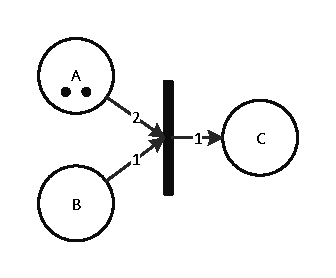
\includegraphics[width=\linewidth]{drawings/Petri1.pdf}
  \caption{Waiting for tokens}\label{fig:petri1}
\endminipage\hfill
\minipage{0.32\textwidth}
  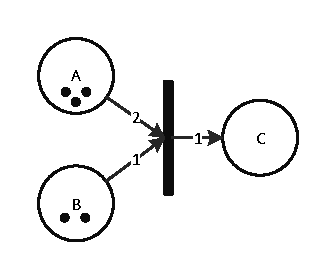
\includegraphics[width=\linewidth]{drawings/Petri2.pdf}
  \caption{Transition ready to fire}\label{fig:petri2}
\endminipage\hfill
\minipage{0.32\textwidth}%
  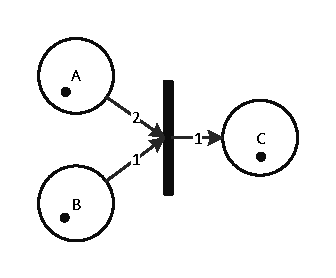
\includegraphics[width=\linewidth]{drawings/Petri3.pdf}
  \caption{After transition fires}\label{fig:petri3}
\endminipage
\caption{Petri net}
\label{fig:petri}
\end{figure}

Petri nets are bipartite directed graphs with two kind of nodes, \emph{places}
and \emph{transitions}.  Connections between the nodes are called \emph{arcs}
and can only connect places to transitions or transitions to places.  Tokens are
held by places and used to represent firing criteria for a transition.  
Figure~\ref{fig:petri} shows a simple example of a Petri net graph.  The 
example defines three places, A, B, and C and one transition.  The firing 
criteria for the transition is two tokens from A and one token from B.  Once 
sufficient tokens arrive, the transition is able to fire, see 
figure~\ref{fig:petri2}.  The transition consumes the two tokens from A and the
one token from B and produces a single token for C, see Figure~\ref{fig:petri3}.

Once formalized into a Petri net, an algorithm can be \emph{unfolded} into an 
occurrence net which represents every specific instance of execution in a flat
linear way.  Once an occurrence net has been defined it can be used to analyze a
concurrent application and prove correctness~\cite{franco2012true}.  We will use 
Petri nets to outline our idealized ray tracing engine for concurrent execution 
on future exascale systems in section~\ref{sec:design}.  

\section{Task-Based Programming Models}
\label{sec:task-based}

One class of programming model that are anticipated to map well onto exascale 
systems are task-based models. They tend to be declarative: An application is
broken down into chunks of work and the inputs and outputs to that work are 
declared in the language semantics. Their explicit data dependencies allow the 
runtime to optimally schedule and execute the tasks, or chunks of work, in the 
application.

Execution can often be further improved by the implementation of a
secondary specification (a file, typically) separate from the program
that provides \emph{hints} to the runtime. The key difference between many
task-based models and more traditional programming models is the
movement from compute-centric to data-centric application design.
Algorithms are designed around the data a task needs to execute and
the data it will produce rather than designed around the computation.

\subsection{The CnC Programming Model}
\label{sec:cnc}

The Concurrent Collections Programming Model (CnC), developed by
Intel, is one such data-centric programming model. Its deterministic
semantics allow a task-based runtime to programmatically exploit
parallelism. In addition, it allows for a secondary file, called a
tuning specification, to provide additional hints that can improve performance.

The CnC model can be thought of as a producer-consumer paradigm where
data is produced and consumed by tasks, or \emph{steps} in CnC
terminology. The produced and consumed data is declared explicitly in
an input file, known as a \emph{graph file}. The steps themselves are
also entities that can be produced. When a step produces another step,
this is known as a \emph{control dependency} and is also declared in the
graph file.

Figure~\ref{fig:cnc_graph} shows a example graph file. The rectangles represent
\emph{step collections}, the ovals represent \emph{data collections} are the
dependencies are the directed edges connecting them. The title of a step
collection is usually a descriptive verb and the title of a data
collection is usually a descriptive noun. The control dependencies are
not shown. A text description of Figure~\ref{fig:cnc_graph} (which
includes control information) is provided to CnC when designing a CnC
application.  Section~\ref{sec:implementation} shows an example of this.

\begin{figure}[t]
  \centering
  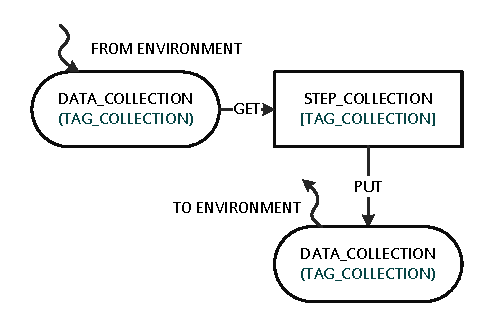
\includegraphics[width=0.5\textwidth]{drawings/CnCExample.pdf}
  \caption{CnC Graph Semantics}
  \label{fig:cnc_graph}
\end{figure}

By declaring all dependencies between steps and data, the specifics
regarding how the algorithm is executed is abstracted out of the
implementation. For example: It is clear what data is needed by a
given step, so if that data has not been produced yet, the step will
not be scheduled. This allows the runtime to optimally decide when and
where to schedule computation. By way of contrast, in a conventional
multithreaded program, it is the responsibility of the programmer to
guarantee that a thread's inputs are available and consequently start
the thread.

For some more complicated semantics, additional hints can be provided
to the runtime through a \emph{tuning specification}. As the tuning
specification usually is in a separate file, this makes it easy to run
the same program on different architectures, as no rewrites of the
application are necessary to switch platforms: just the tuning
specification.

\subsubsection{Language Specifics}
\label{sec:cnc_language}

The CnC model is built on three key constructs; step collections, data
collections, and control collections ~\cite{budimlicconcurrent}. A
step collection defines computation, an instance of which consumes and
produces data. The consumed and produced data items belong to data
collections. Data items within a data collection are indexed using
item epmh{tags}: tuples that, like primary keys, can uniquely identify a
data item in the data collection. Finally, the control collection
describes the prescription, or creation, of step instances. The
relationship between these collections as well as the collections
themselves are defined in the graph file.

Developing a CnC application then begins with designing the graph
file. An algorithm is broken down into computation steps, instances of
which correspond to different input arguments. These steps, along with
the data collections become nodes, in the graph. Each step can
optionally consume data, produce data, and/or prescribe additional
computation. These relationships: producer, consumer, and control,
define the edges of the graph and will dynamically be satisfied as the
program executes.

The next and final required step in producing a CnC application is to
implement the step logic. The flow within a single step is: consume,
compute, and produce. This ordering is required as there is no
guarantee the data a step needs will be ready when the step begins
executing. This is due to steps being preemptively scheduled when they
are prescribed. Most of the time the data \emph{will} be ready when a
step begins execution, but occasionally and often due to an
implementation error, a step's data may never be available.
Internally, if the data is not ready when a step begins execution
it will halt execution and try again later. To improve performance,
hints can be provided through the tuning specification to increase the
likelihood that steps are schedule for execution when their required
input data is ready.

\subsection{Example}
\label{sec:cnc_example}

\begin{figure}[!tb]
  \centering
  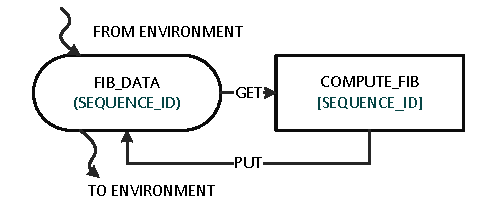
\includegraphics[width=0.5\textwidth]{drawings/FibExample.pdf}
  \caption{A CnC Graph to Compute the Fibonacci Sequence}
  \label{fig:fib_graph}
\end{figure}

Figure~\ref{fig:fib_graph} shows an example of a
simple iterative implementation of the Fibonacci sequence. This
application consists of one step, COMPUTE\_FIB, which takes the
previous two computed values as input and produces the next value in
the sequence. One data collection, FIB\_DATA, exists for the
application. Data within the collection is indexed by a tag consisting
of the sequence number. Tags 1-5, then index the values 1,
1, 2, 3, 5, respectively. The first two values of the data collection
are produced by the environment, the rest of the values in the
collection are produced as needed by COMPUTE\_FIB. A tag exists for
COMPUTE\_FIB as well. We can index this collection by the integer
sequence a particular instance will produce. For example, the step
% RRL: What do you mean by "integer sequence"? The *whole* Fib sequence?
instance at tag 3 will consume the data at tag 1 and 2, and produce
data at tag 3. Specifically it will consume 1, 1 and produce 2.
The number of steps executed in this example is provided by the 
environment.

\section{Distributed and Parallel Ray Tracing}
\label{sec:ray_tracing}

\emph{"Ray tracing is the future and ever will be"} was the title of a SIGGRAPH 
course in 2013.  The course outlined the state of the art in ray tracing 
technology, covering recent developments and optimization techniques to speed up 
the core algorithm such as acceleration data structures.  This quote points out 
that although we have optimized ray tracing to a T, it is still not the primary
rendering technique used in graphics.  This section outlines key strategies for 
ray tracing optimization with an emphasis on parallel and distributed 
advancements.

Ray tracing is an application that tends to scale well as you subdivide the 
task.  Each ray cast into a scene does not need any information about any other 
ray cast into the scene.  Communication between rays, therefore, is non-existent 
and only the cost of creating new tasks and joining the tasks to produce the 
final ray traced image limit the amount of parallelism you can extract from the
algorithm\footnote{ %
  The system you are executing a ray tracer on limits the parallelism of the 
  application.  
}.

Although no ray depends on any other ray in a ray tracing algorithm, the data 
needed by each individual ray varies widely as its path is traced. Acceleration 
structures such as k-d trees have been developed to increase ray tracing 
performance. As the size of the scene increases, however, it is no longer 
possible to store an entire data set in an acceleration structure in shared 
memory.

One solution is to implement data decomposition. Each node on a distributed 
system is then responsible for a subset of the domain. Primary, secondary, 
and subsequent rays are then communicated across nodes as the algorithm 
executes. These types of models typically rely on expensive pre-processing steps 
that help to balance both the data distribution and rendering work evenly across 
nodes ~\cite{navratil2014dynamic}.

Load balancing, a significant bottleneck on today's systems, may not be easily 
implemented on exascale systems. The proposed smarter programming models and 
runtimes, on the other hand, will allow for scheduling and data movement 
decisions to be made at runtime which will help reduce imbalance in a system. 
Data and computation can be dynamically migrated off of overworked nodes 
assuming a properly sized granularity for tasks and data.

\section{Embree}
\label{sec:embree}
Embree is a parallel ray tracing library developed at Intel that has been 
optimized at the architecture level to take advantage of chip specific caching 
and communication.  Embree supports both packet (multiple rays) and single ray 
intersection queries into optimized data structures ~\cite{wald2014embree}. The 
data structures used in Embree are BVH or bounding volume hierarchy structures.  
BHV data structures are hierarchical structures that are fast to build with 
small memory footprints and fast traversal times due to their shallow depth 
~\cite{wald2014embree}.  Due to the optimization within Embree, the library 
exploits on node parallelism and is on par with other state of the art ray 
tracing libraries. 

%%% Local Variables: 
%%% mode: latex
%%% TeX-master: "main"
%%% End: 
